%\chapter{Data Analysis}\label{chap:03}

\section{Analysis Strategy}
This analysis searches for a spin-1 \(Z^{\prime}\) resonance (\(m_{Z^{\prime}} = 0.5-3\,\mathrm{TeV}\)) decaying to \(t\bar{t}\) pairs. The lepton+jets channel was selected for its optimal balance of branching fraction (\(\sim\)30\%), manageable backgrounds, and compatibility with single-lepton triggers. 

\textbf{Data and Simulation:}
\begin{itemize}
    \item \textit{Data:} \(pp\) collisions at \(\sqrt{s} = 13\,\mathrm{TeV}\) (\( \mathcal{L} = 1\,\mathrm{fb}^{-1}\)) with single-lepton triggers (\(E_T > 25\,\mathrm{GeV}\) for \(e\), \(p_T > 25\,\mathrm{GeV}\) for \(\mu\))
    \item \textit{Backgrounds:} Simulated \(t\bar{t}\), single-top, \(W/Z\)+jets, and diboson processes
    \item \textit{Signal:} Simulated narrow-width \(Z^{\prime}\) (\( \Gamma/m \sim 1\%\)) at benchmark masses (0.5, 0.7, 1.0, 1.5, 2.0, 3.0 TeV) with SM-like couplings
\end{itemize}

\textbf{Reconstruction and Selection:}
\begin{itemize}
    \item \textit{Objects:} Isolated leptons (\(p_T > 25\,\mathrm{GeV}\)), anti-\(k_t\) jets (\(R=0.4\), \(p_T > 25\,\mathrm{GeV}\)), \(b\)-tagging (70\% WP), and \(E_T^{\mathrm{miss}} > 20\,\mathrm{GeV}\)
    \item \textit{Event selection:} Exactly 1 lepton, \(\geq\)4 jets (2 \(b\)-tagged), \(m_T(W) > 30\,\mathrm{GeV}\)
    \item \textit{Top reconstruction:} Hadronic top (3 jets, 1 \(b\)-tagged) and leptonic top (lepton + \(E_T^{\mathrm{miss}} + b\)-jet)
\end{itemize}

\textbf{Discriminant:} The reconstructed \(t\bar{t}\) invariant mass \(m_{t\bar{t}}\) serves as the final observable for resonance identification.

\section{Selection Cuts}

The event selection follows a sequential cut flow implemented in \texttt{runSelection.C}. The applied cuts are:

\vspace{-0.5\baselineskip}
\begin{table}[h]
\centering
\begin{tabular}{|c|l|c|}
\hline
\textbf{Step} & \textbf{Selection Criteria} & \textbf{Value} \\ \hline
1 & Exactly one lepton & \texttt{lep\_n = 1} \\ \hline
2 & Lepton transverse momentum & $p_T > 50$ GeV \\ \hline
3 & Lepton pseudorapidity & $|\eta| < 2.5$ \\ \hline
4 & Jet multiplicity & $3 \leq N_{\mathrm{jets}} \leq 5$ \\ \hline
5 & Leading jet $p_T$ threshold & $\geq$90 GeV \\ \hline
6 & $b$-tagging requirement (MV2c10) & $> 0.83$ \\ \hline
7 & Missing transverse energy & $E_T^{\mathrm{miss}} > 40$ GeV \\ \hline
\end{tabular}
\end{table}
\vspace{-0.5\baselineskip}

\autoref{fig:histo} shows the cumulative efficiency after these cuts. Background processes (especially $t\bar{t}$) experience significant suppression, though data reduction suggests no strong signal presence.

\begin{figure}[H]
       %\setkeys{Gin}{draft=false}
	\centering
	\fcolorbox{black}{white}{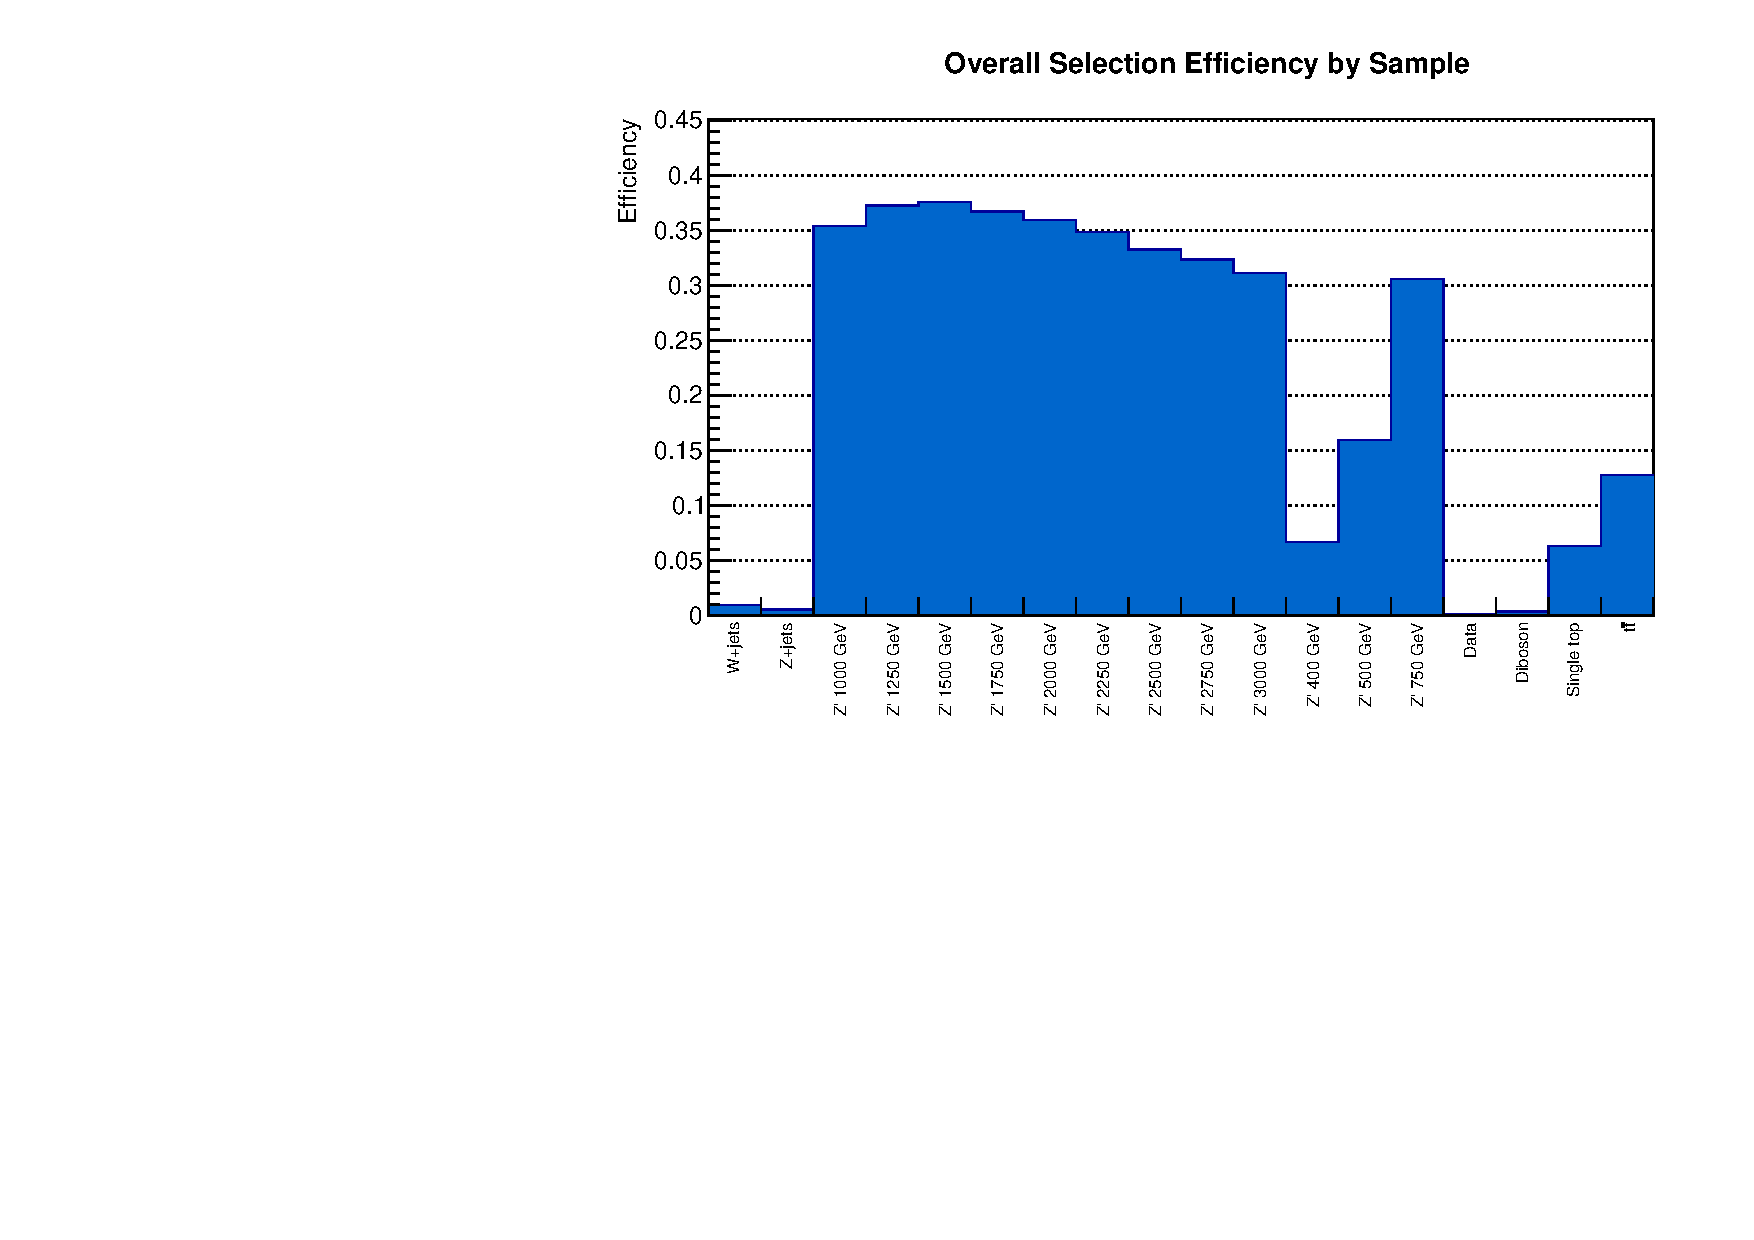
\includegraphics[scale=0.6]{graphs/efficiency_histogram.pdf}}
	\caption{Overall efficiency result of the cuts on all samples.}
	\label{fig:histo}
\end{figure}

\section{Fundamental distributions}

The dominant background after event selection is strong $t\bar{t}$ production due to its identical final state to the signal, resulting in high selection efficiency. Kinematic distributions for the $t\bar{t}$ sample were examined, including:
\begin{itemize}
    \item Lepton properties: $p_T$, $\eta$, $\phi$, $E$
    \item Jet properties: $p_T$, $\eta$, $\phi$, $E$ for all jets and leading jets
    \item Multiplicities: Number of jets and $b$-tagged jets
    \item Missing transverse momentum ($p_{T,\text{miss}}$)
\end{itemize}

\begin{figure}[H]
       %\setkeys{Gin}{draft=false}
	\centering
	\fcolorbox{black}{white}{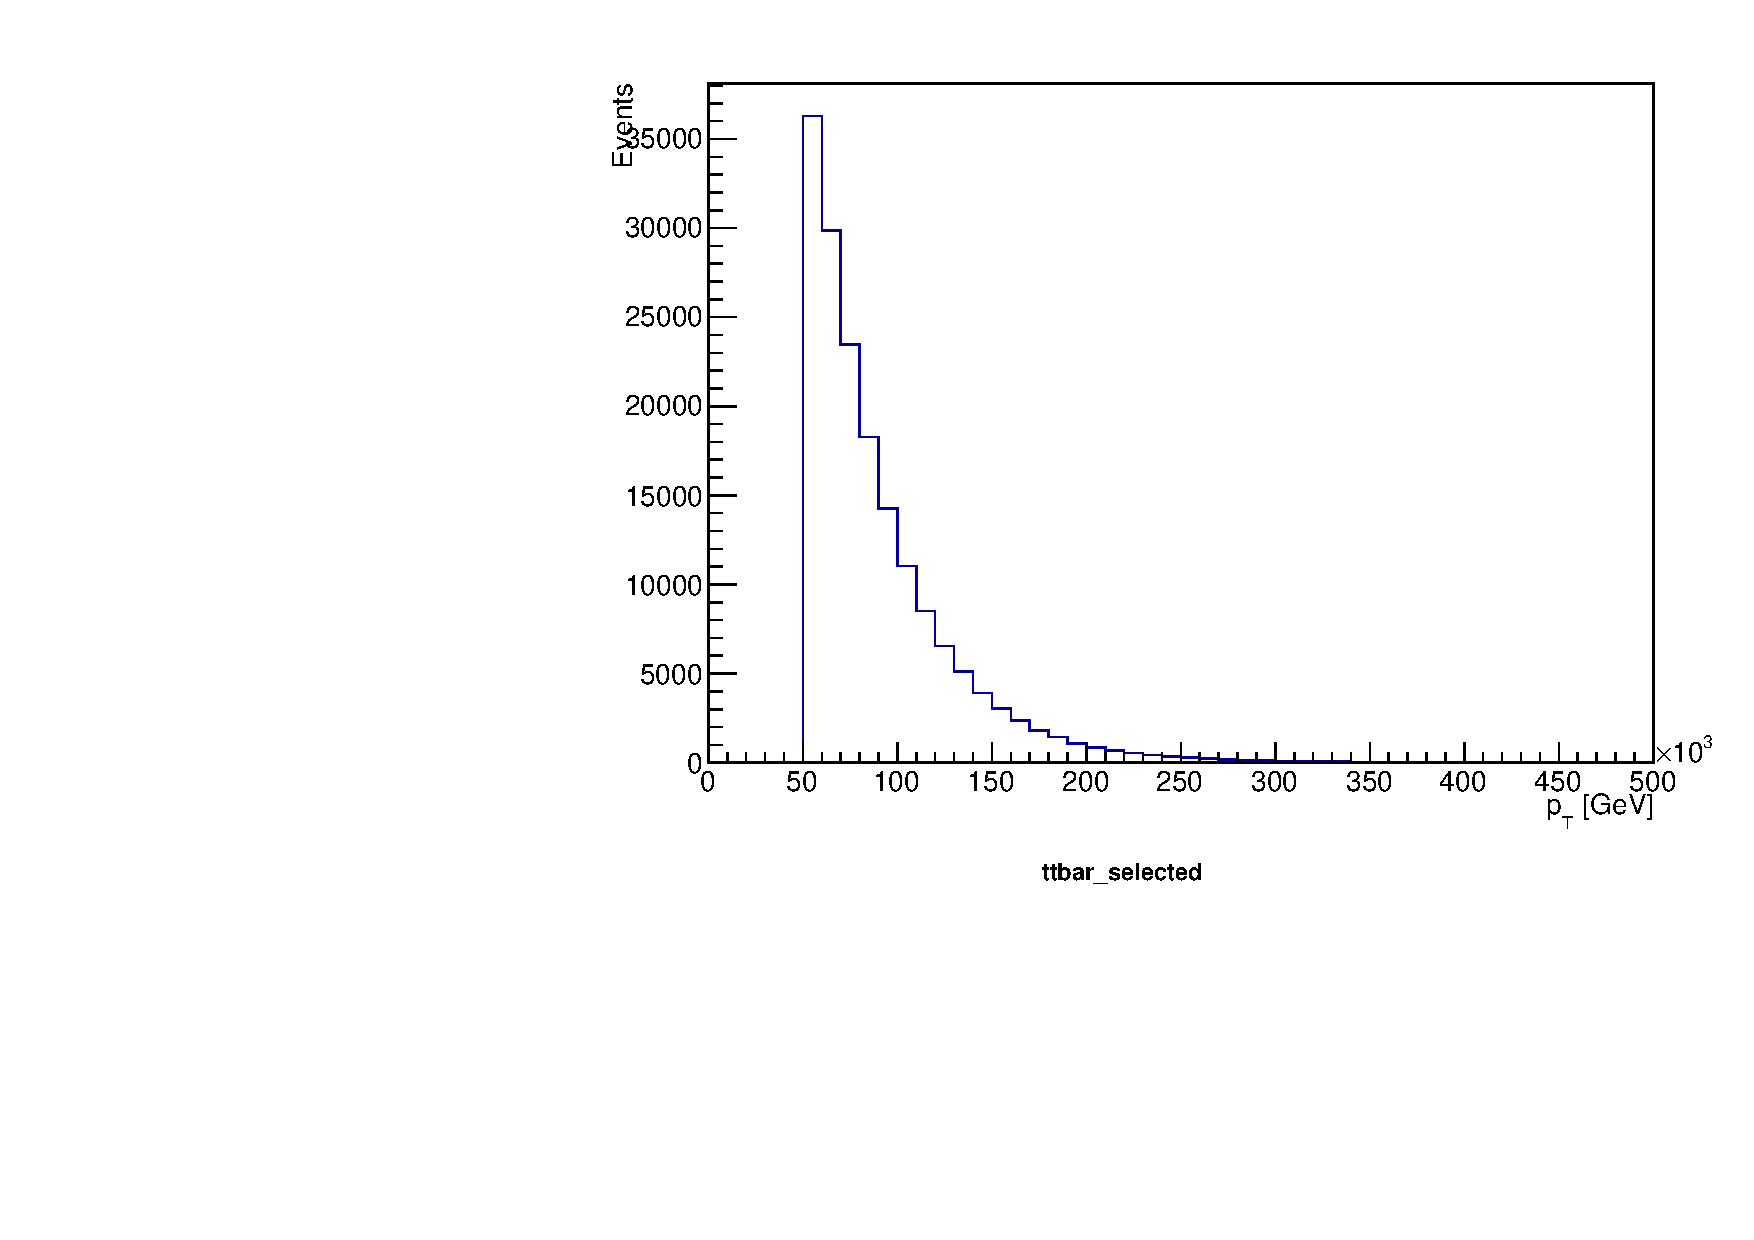
\includegraphics[scale=0.5]{graphs/sec04/lep_pt_ttbar_selected.pdf}}
	\caption{Lepton transverse momentum.}
	\label{fig:lep_pt}
\end{figure}

\begin{figure}[H]
       %\setkeys{Gin}{draft=false}
	\centering
	\fcolorbox{black}{white}{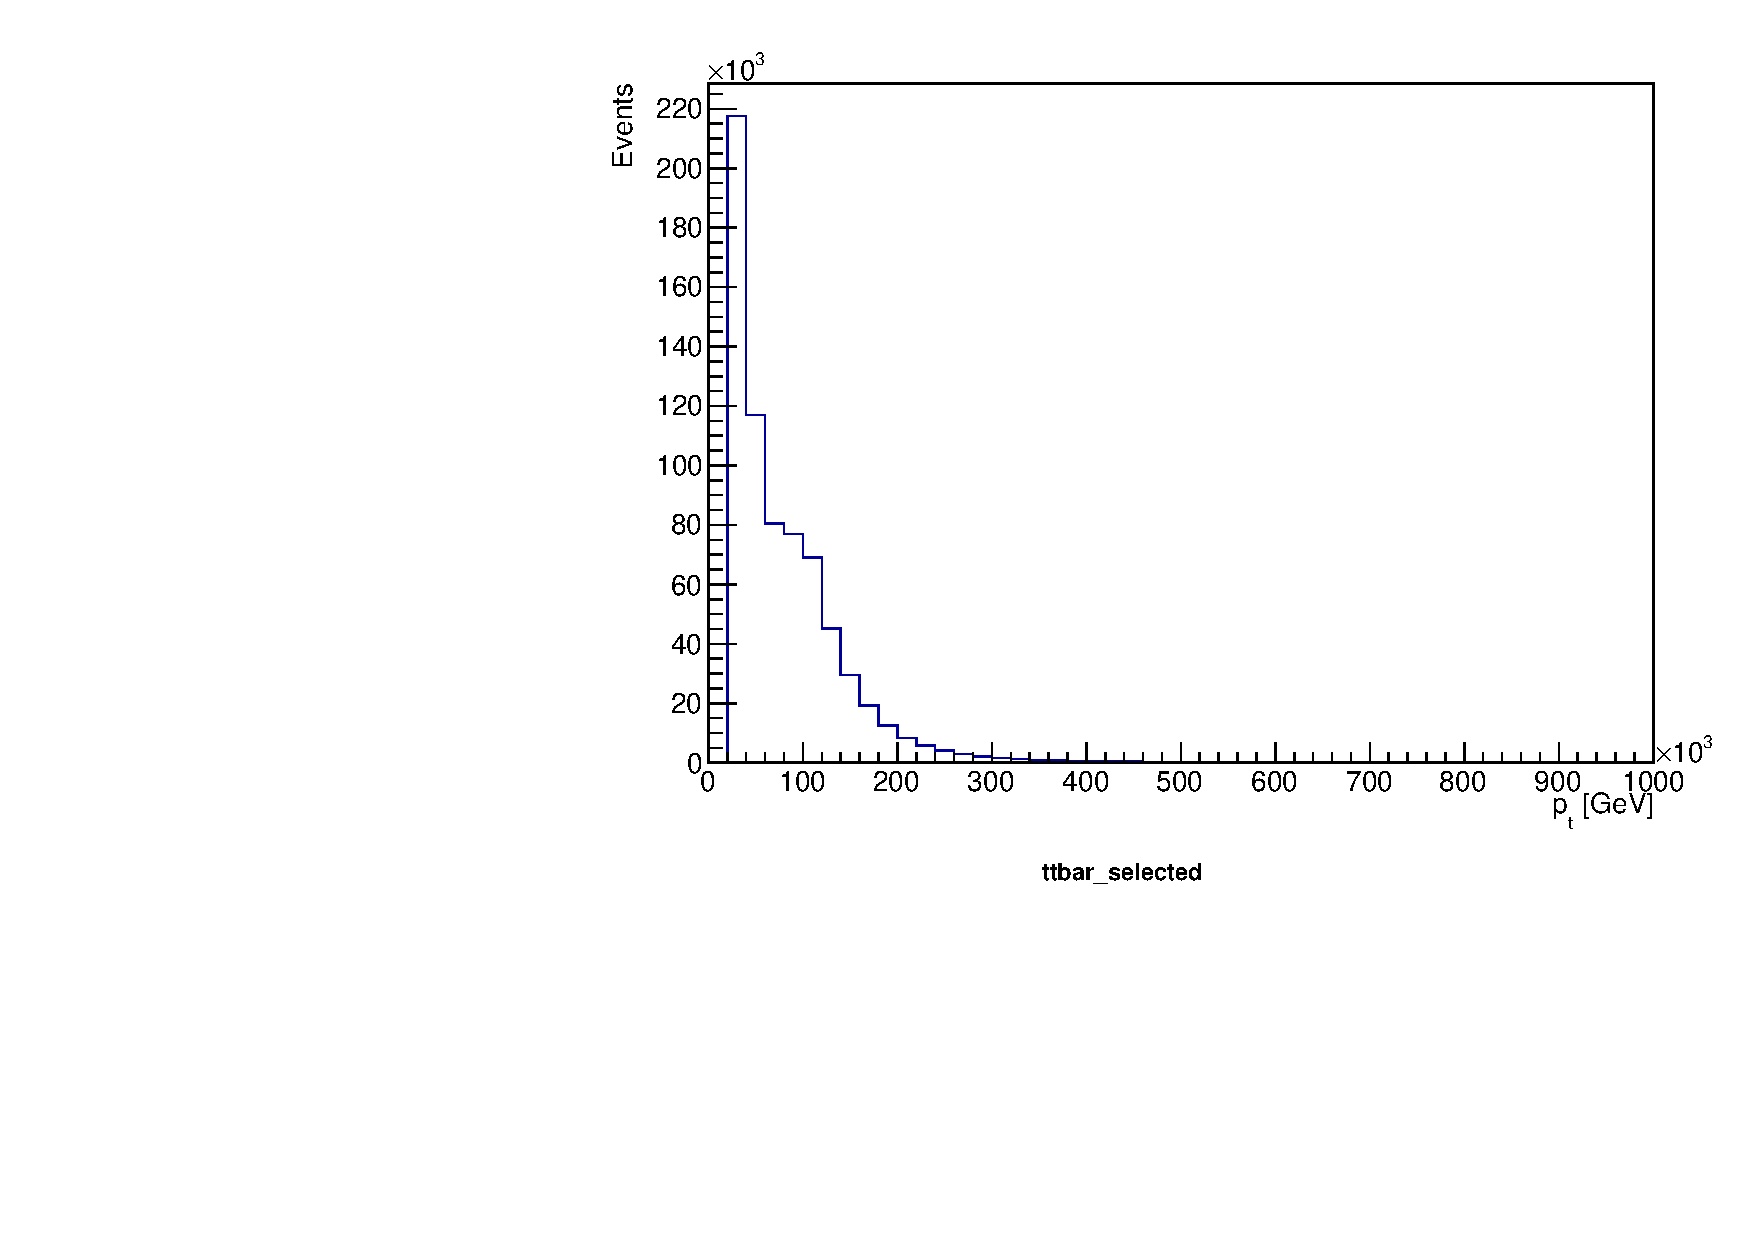
\includegraphics[scale=0.5]{graphs/sec04/jet_pt_ttbar_selected.pdf}}
	\caption{Jet transverse momentum.}
	\label{fig:jet_pt}
\end{figure}

Both lepton and jet $p_T$ exhibit exponential decays, while Jet and $b$-jet multiplicities show similar distributions.

All distributions align with SM expectations, confirming background modeling validity. Consequently, these observables alone cannot serve as
the final discriminant in a resonance search.

\section{Discriminant}

To enhance the signal-to-background separation in the search for $t\bar{t}$ resonances, multiple kinematic discriminants were investigated. These discriminants leverage the full event topology by combining four-vectors of reconstructed objects. The primary candidates considered were:

\begin{itemize}
    \item Missing transverse momentum ($p_{\mathrm{T, miss}}$)
    \item Azimuthal angle separation between $p_{\mathrm{T, miss}}$ and the lepton ($\Delta\phi(\ell, p_{\mathrm{T, miss}})$)
    \item Invariant mass of the three highest-$p_T$ jets ($m(3j)$)
    \item Invariant mass of the reconstructed $t\bar{t}$ system ($m_{t\bar{t}}$), formed by:
    \begin{align*}
        m_{t\bar{t}} = m(4j, \ell, \nu) = m(p_{t_{\mathrm{had}}} + p_{t_{\mathrm{lep}}})
    \end{align*}
    \item Pseudorapidity of the full $t\bar{t}$ system ($\eta(4j, \ell, \nu)$)
\end{itemize}

Distributions of these variables were compared between simulated $t\bar{t}$ background and $Z'$ signal events (e.g., $m_{Z'} = 1000$\,GeV). While $\Delta\phi$, $m(3j)$, and $\eta(4j, \ell, \nu)$ exhibited similar shapes for both samples (with larger fluctuations in the $Z'$ sample due to limited statistics), the $p_{\mathrm{T, miss}}$ distribution showed an exponential decrease for background but no clear functional form for signal. Crucially, $m_{t\bar{t}}$ displayed fundamentally different behavior: 

\begin{itemize}
    \item For background, a broad peak near 500\,GeV (higher than the expected $2m_t \approx 346$\,GeV, suggesting MC modeling limitations)
    \item For $Z'$ signal, a sharp resonance at the generated mass (e.g., $\sim$1100\,GeV for $m_{Z'} = 1000$\,GeV)
\end{itemize}

The reconstructed $m_{t\bar{t}}$ demonstrated superior discrimination power due to its direct physical interpretation: it should peak at the resonance mass for a $Z' \to t\bar{t}$ signal while yielding a smoothly falling distribution for SM backgrounds (\autoref{fig:invMass03}). This clear signature motivated its selection as the final discriminant for statistical analysis in both studies. Other variables served auxiliary roles in validation and systematic uncertainty studies but lacked comparable sensitivity to narrow resonances.

\begin{figure}[H]
       %\setkeys{Gin}{draft=false}
	\centering
	\fcolorbox{black}{white}{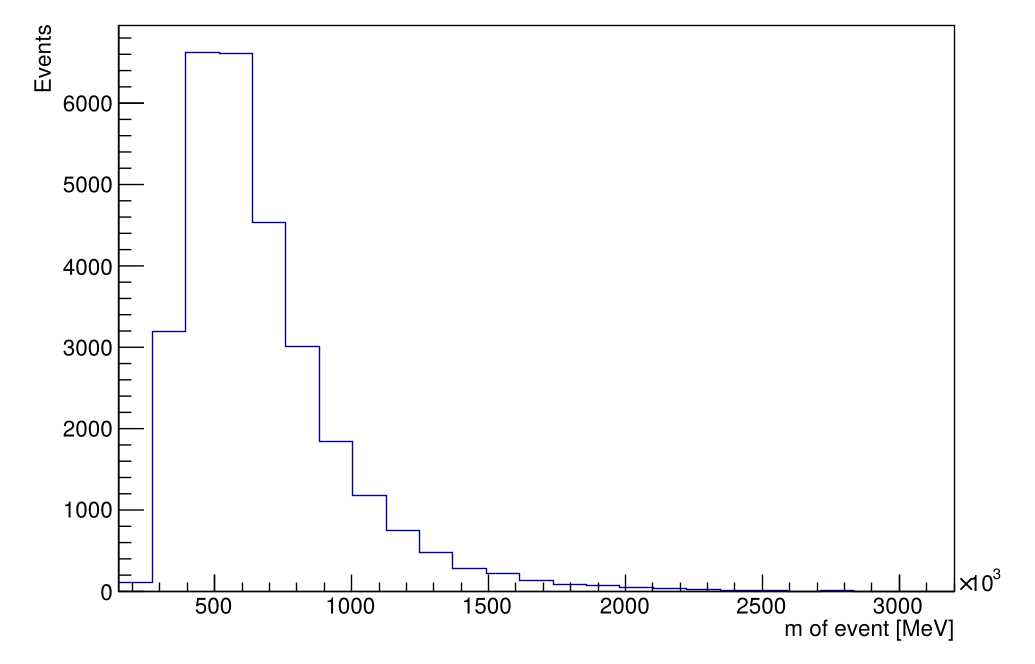
\includegraphics[scale=0.3]{graphs/invMassTT04.png}}
	\caption{Reconstructed invariant mass of the four jets with the highest transverse momentum, the lepton, and missing transverse momentum ($m_{t\bar{t}}$) for SM background.}
	\label{fig:invMass03}
\end{figure}

\begin{figure}[H]
       %\setkeys{Gin}{draft=false}
	\centering
	\fcolorbox{black}{white}{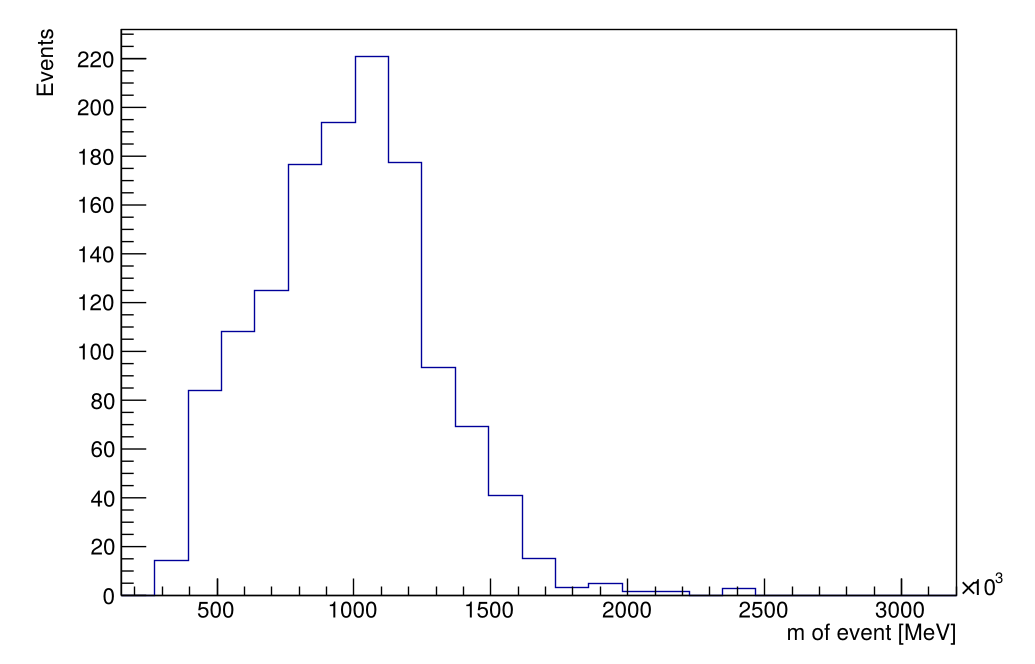
\includegraphics[scale=0.3]{graphs/invMassZ03.png}}
	\caption{Reconstructed invariant mass of the four jets with the highest transverse momentum, the lepton, and missing transverse momentum for $Z'$ signal ($m_{Z'} = 1000$\,GeV).}
	\label{fig:invMass04}
\end{figure}

\subsection{Data-Monte Carlo Agreement Validation}
\label{subsec:data_mc_agreement}

Prior to conducting the resonance search, rigorous validation of the agreement between collision data and Monte Carlo (MC) simulations is essential. This verification ensures the reliability of background modeling in control regions and establishes confidence in the statistical interpretation framework. The validation procedure comprises two complementary approaches:

\begin{enumerate}
    \item \textbf{Event Yield Comparison:} 
    The expected event yields for Standard Model (SM) processes are calculated as:
    \[
    N_{\text{expected}} = \mathcal{L} \cdot \sigma \cdot (A \cdot \epsilon)
    \]
    where \(\mathcal{L}\) denotes the integrated luminosity, \(\sigma\) the process cross-section, and \((A \cdot \epsilon)\) the selection efficiency. For the dataset, an excess of observed events compared to the expected number is observed. This discrepancy persists across kinematic distributions but lacks a resonant mass peak, suggesting systematic mismodeling rather than new physics.
    
    \item \textbf{Kinematic Distribution Analysis:} 
    Stacked histograms compare data and MC distributions for key observables, normalized using per-event weights:
    \[
    w = \frac{\text{generator weight} \times \mathcal{L} \times \sigma}{\sum \text{generator weights}}.
    \]
    Lower plots display the data/MC ratio with statistical uncertainties. Results show:
    \begin{itemize}
        \item \textit{Lepton \(p_T\)}: Agreement within \(\pm 20\%\) across \(p_T\) bins, with minor deviations \(>200\;\text{GeV}\) consistent with statistical fluctuations.
        \item \textit{Reconstructed \(m_{t\bar{t}}\)}: Smoothly falling spectrum with discrepancies between Data and MC reconstruction.
    \end{itemize}
\end{enumerate}

\noindent Indeed for the mass distribution can be spotted some deviations (e.g. around 635 GeV and 900 GeV) that suggest for a shift in the Data distribution more to the right. The observed yield excess is attributed to limitations in MC simulations (e.g., imperfect \(b\)-tagging efficiency modeling or parton shower tuning) rather than a signal. This validation justifies proceeding to statistical analysis of the final discriminant.

We therefore conclude that the background modeling is reliable in the control regions, and proceed to inspect the final mtt̄ spectrum for evidence of a signal. Just by looking at it, we do not see any indication of a signal.

\begin{figure}[H]
       %\setkeys{Gin}{draft=false}
	\centering
	\fcolorbox{black}{white}{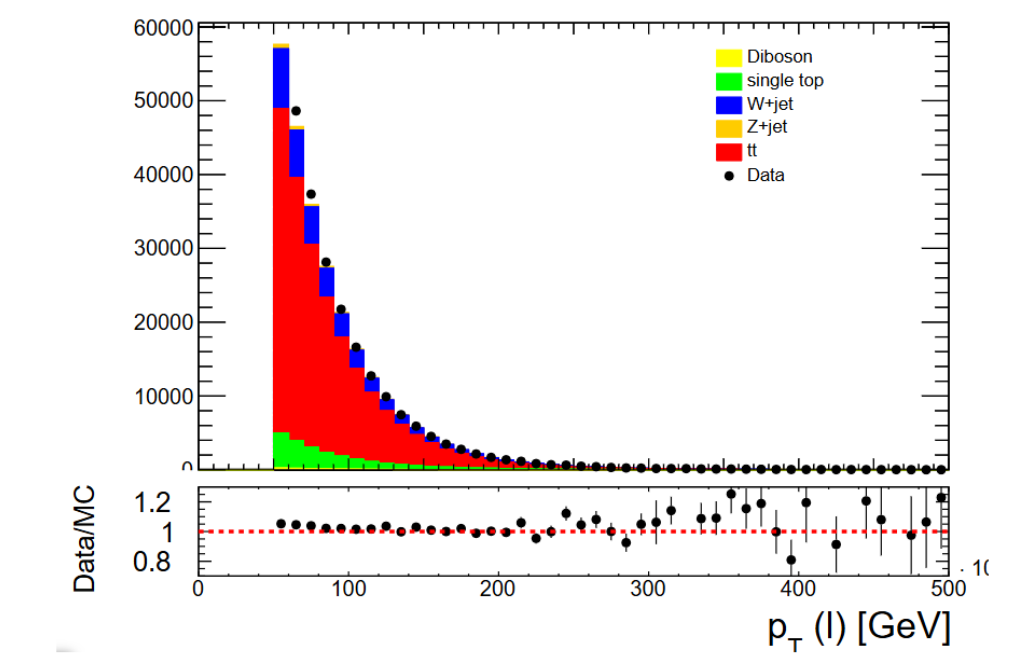
\includegraphics[scale=0.3]{graphs/agree01.png}}
	\caption{Stacked comparisons of lepton $p_T$ and between data and MC. The lower panel shows the data/MC ratio with statistical uncertainties.}
	\label{fig:ag01}
\end{figure}

\begin{figure}[H]
       %\setkeys{Gin}{draft=false}
	\centering
	\fcolorbox{black}{white}{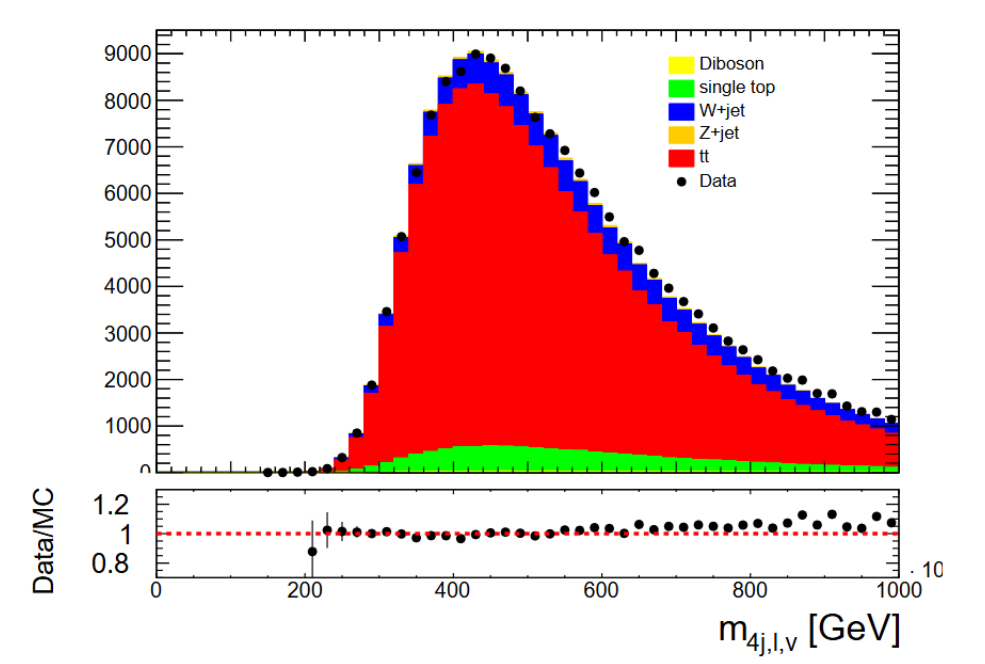
\includegraphics[scale=0.3]{graphs/agree02.png}}
	\caption{Stacked comparisons of reconstructed $m_{t\overline{t}}$ between data and MC.}
	\label{fig:ag02}
\end{figure}

\section{Statistical Analysis}

The agreement between observed data and simulated Standard Model (SM) background predictions was quantified using the $\chi^2$ test statistic. For the final discriminant variable (reconstructed $t\bar{t}$ invariant mass $m_{t\bar{t}}$), the $\chi^2$ value is computed as:
\[
\chi^2 = \sum_{i=1}^{N_{\text{bins}}} \frac{(N_{\text{data}}^i - N_{\text{MC}}^i)^2}{N_{\text{MC}}^i}
\]
where $N_{\text{data}}^i$ and $N_{\text{MC}}^i$ represent event counts in bin $i$ for data and simulated background, respectively. The corresponding $p$-value is derived from the $\chi^2$ distribution with $k = N_{\text{bins}} - 1$ degrees of freedom.\\

A $p$-value below $2.7\times 10^{-3}$ (3$\sigma$) is considered an \emph{evidence}, while a $p$-value below $5.7\times 10^{-7}$ (5$\sigma$) is considered an \emph{observation}.

The calculated $p$-value of $1.34 \times 10^{-2}$ indicates a deviation of approximately $2\sigma$. This value is above the conventional threshold and thus does not constitute significant evidence for a signal above the background. Furthermore, this statistical analysis does not incorporate systematic uncertainties, which, as discussed in the following section, may substantially influence the final result.

\subsection{Incorporating Systematic Uncertainties}

To quantify systematic uncertainties, the $\chi^2$ test was recomputed with a uniform 14\% per-bin uncertainty. This comprehensive uncertainty combines:
\begin{itemize}
    \item 4\% integrated luminosity uncertainty
    \item 10\% experimental uncertainties (from $b$-tagging efficiency, lepton identification, etc.)
\end{itemize}
The modified bin variance accounts for these systematics through:
\[
\sigma_{\text{tot}}^2 = \sigma_{\text{stat}}^2 + (0.14 \times N_{\text{bkg}})^2
\]
where $\sigma_{\text{stat}}$ is the statistical uncertainty and $N_{\text{bkg}}$ is the background yield per bin.

This leads to a p-value equal to 0.998: no $Z'$ boson was so discovered.

\subsection{Exclusion Limits at 95\% Confidence Level}

In the absence of statistically significant evidence for a signal, we derive 95\% confidence level (CL) upper limits on the production cross section times branching ratio \(\sigma(pp \to Z') \times \mathcal{B}(Z' \to t\bar{t})\). For each hypothesized resonance mass \(m_{Z'}\), we introduce a signal template superimposed on the SM background and systematically vary its normalization. The normalization is adjusted until the \(\chi^2\) probability comparing data to the combined background-plus-signal model falls below 0.05 (i.e., \(1 - 0.95\)). The resulting exclusion curve (\enquote{observed limit}) is plotted against theoretical predictions, as shown in \autoref{fig:chi}.

\begin{figure}[H]
       %\setkeys{Gin}{draft=false}
	\centering
	\fcolorbox{black}{white}{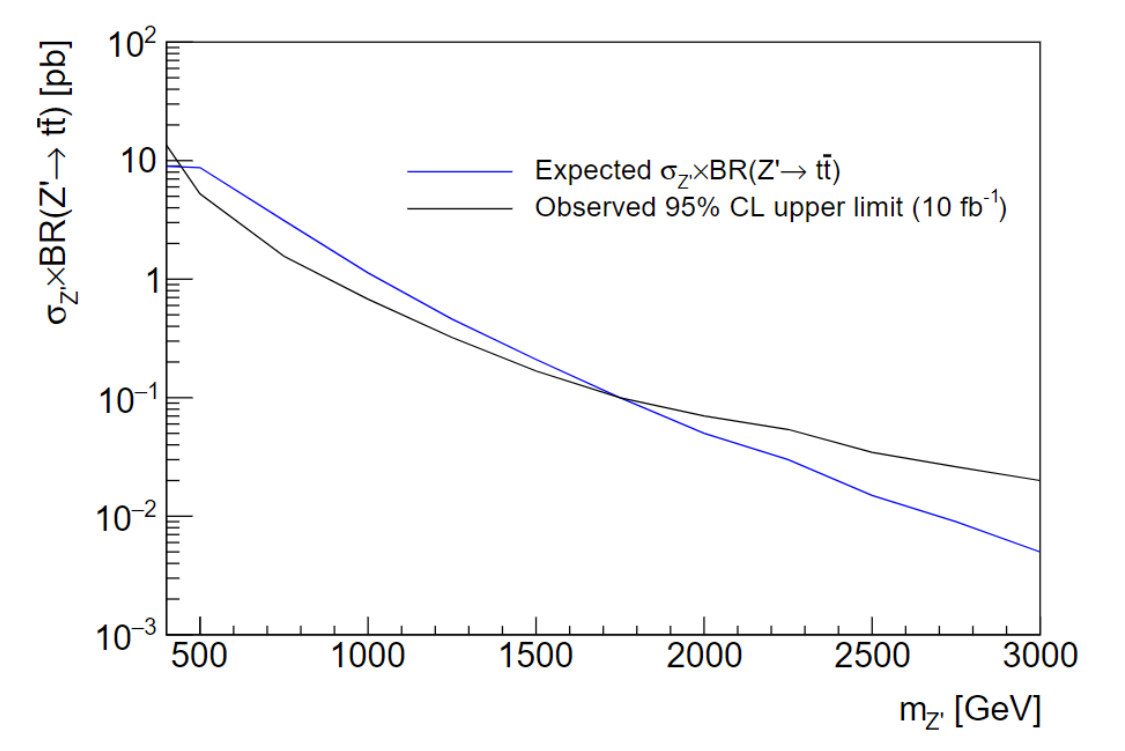
\includegraphics[scale=0.3]{graphs/chi.png}}
	\caption{Theoretical limits and 95\% CL exclusion limits on the production cross section for different $Z'$ boson masses.}
	\label{fig:chi}
\end{figure}

\begin{itemize}
    \item \textbf{Expected limit (blue curve)}: The median upper limit under the background-only hypothesis (no true \(Z'\) signal), quantifying the analysis sensitivity to a narrow resonance of mass \(m_{Z'}\) given statistical fluctuations of SM backgrounds.
    \item \textbf{Observed limit (black curve)}: Actual upper limits derived from collision data. Fluctuations in data relative to expectations shift this curve above/below the expected limit.
\end{itemize}

The vertical axis, shown on a logarithmic scale, represents the fraction of the $Z'$ production cross section corresponding to the \texorpdfstring{$Z' \rightarrow t\overline{t}$}{} decay channel, expressed in pb. The horizontal axis denotes the hypothesized $Z'$ boson mass, scanned from 500 GeV to 3 TeV.

The expected limit (blue curve) represents the median expected 95\% confidence level (CL) upper limit under the background-only hypothesis, where no $Z'$ signal is present. This curve characterizes the intrinsic sensitivity of the analysis to a narrow resonance of a given mass $m_{Z'}$. The observed limit (black curve) shows the actual 95\% CL upper limit derived from the experimental data.

Statistical fluctuations in the data cause the observed limit to deviate from the expected median. An upward fluctuation of the signal-like background results in an observed limit less stringent than expected (i.e., above the blue curve), while a downward fluctuation yields a more stringent limit (i.e., below the blue curve).

This plot provides a direct means of evaluating theoretical models. For example, if any model that predicts values of $\sigma \times \mathcal{B}$ exceeding the black \enquote{observed} curve, then it is excluded at the 95\% confidence level. As an example, consider a benchmark Sequential Standard Model $Z'$ with a mass of $m_{Z'} = 2$ TeV , which predicts $$\sigma \times \mathcal{B} \approx 0.2 \hspace{1.5pt} \text{pb}$$
\noindent
If the observed upper limit at 1 TeV is 0.1 pb, this specific model prediction would be excluded by the analysis.